% !TEX program=xelatex
% !TEX options=-synctex=1 -shell-escape -interaction=nonstopmode -file-line-error "%DOC%"
\documentclass[zihao=-4,fontset=fandol]{ctexart}
\usepackage[hmargin=2cm,vmargin=2.4cm]{geometry}
\usepackage{amsmath,amssymb}
\usepackage{hologo}
\usepackage[many]{tcolorbox}
\usepackage[color,tikz]{texhigh}

%% if WSL use host font (windows font), \kaomoji would be much slower,
%% if not, just delete these lines.
\csname file_if_exist:nT\endcsname {/mnt/c/Windows/Fonts/arial.ttf}{%
  \wlog{I found the code is running on WSL, I will redefine \string\kaomoji.}
  \NewCommandCopy\orikaomoji\kaomoji
  \DeclareDocumentCommand\kaomoji{sO{}m}{\IfBooleanTF{#1}{\orikaomoji*[#2]{#3}}{\orikaomoji*[fontsize=50bp,#2]{#3}{\includegraphics[height=10bp]}}}
}

\usepackage[colorlinks]{hyperref}
\ifdefined\xeCJKsetup
  \SetKeys[texhigh/high]{
    font=\ttfamily\xeCJKsetup{CJKecglue={\hskip 0pt plus 0.08\baselineskip}}\raggedright,
  }
\else
  \SetKeys[texhigh/high]{
    font=\ttfamily\raggedright,
  }
\fi
\newfontfamily\emojifont{Noto Emoji}
% 若系统没有这些字体会自动忽略
\SetKeys[texhigh/layout]{fonts={Segoe UI,Segoe UI Symbol,Arial,Microsoft YaHei UI,PingFang SC,FandolHei}}
\SetKeys[texhigh/high]{cache-dir=texhigh-cache/, % cache-dir 不要忘记加 /,注意:需要先创建 texhigh-cache 文件夹!!
  cs-category*={texhigh}{^.{0,3}?texhigh.+|^TH.+|^TeXHigh$|^kaomoji$}{\THPASS}}
\tcbset{listing engine=texhigh, listing file=texhigh-cache/\jobname.listing}
\newcounter{example}
\newtcblisting[use counter=example, number format=\arabic]
  {examcode}[2][]{listing and text, 
  title=代码 \thetcbcounter, enhanced,
  comment={#2},
  left=2mm, right=2mm, top=2mm, bottom=2mm,
  sharp corners=downhill, arc=12pt, %skin=bicolor,
  fontupper=\linespread{1}\selectfont, left=6pt,
  colback=blue!1!white, colframe=blue!75!black,colbacklower=white,
  segmentation style={draw=blue,thick,solid},
  attach boxed title to top right={yshift=-\tcboxedtitleheight},
  boxed title style={
    colframe=blue!75!black,colback=blue!15!white,
    sharp corners=downhill,arc=12pt,
  },
  coltitle=blue!90!black, fonttitle=\bfseries,
  before skip balanced=2bp plus .5\baselineskip,
  after skip balanced=2bp plus .5\baselineskip,
  breakable,
  #1
}
\ProvideDocumentCommand{\cs}{m}{\texttt{\textbackslash\detokenize{#1}}}
\ProvideDocumentCommand{\meta}{m}{\ensuremath\langle\textit{#1}\ensuremath\rangle}
\ProvideDocumentCommand{\oarg}{m}{\texttt[\meta{#1}\texttt]}
\ProvideDocumentCommand{\marg}{m}{\texttt\{\meta{#1}\texttt\}}
\begin{document}

\title{高亮 \TeX 和 \LaTeX3 代码——使用\textsf{texhigh} 宏包}
\author{雾月\thanks{longaster@163.com}}
\date{\today\quad v0.3.2}
\maketitle

\textsf{texhigh} 宏包\footnote{\url{https://github.com/Sophanatprime/texhigh}}%
是专用来高亮 \TeX 文件的宏包。基于由 Rust 编写的命令行工具
texhigh\footnote{\url{https://github.com/Sophanatprime/texhigh-rs}},
处理 1.29MB 左右(39,300 余行)的 \texttt{expl3-code.tex} 只需 0.18s 左右
(操作系统为 Windows,CPU 为 i7-12700H),
处理速度约为 \textsf{minted} 宏包使用的 pygmentize(约 3.4s)的 19 倍,
texhigh 的增强模式也比它快 10 到 16 倍(约 0.21s)。
对于普通大小的 \TeX 代码,处理它们所需的时间相比于 \TeX 文件本身编译所需的时间,
已经可以忽略不记。

\textsf{texhigh} 主要是在 \LaTeX 中为 texhigh 命令行工具提供交互接口。这要求在编译 \TeX
文件时启用 \texttt{--shell-escape}。

texhigh 除了可用于高亮 \TeX 文件,还支持计算文字的布局。
基于此特性,\textsf{texhigh} 提供了输出颜文字的功能:
\kaomoji{ε(┬┬﹏┬┬)3} ,只需使用 \texhighverb{\kaomoji}\texttt\{\ensuremath{\langle}\verb|颜文字|\ensuremath{\rangle}\texttt\}。
默认使用系统字体,也可自行设置 \kaomoji{ヾ(≧▽≦*)o}。

% https://emojicombos.com/cute-kaomoji
\kaomoji{ଘ(੭*ˊᵕˋ)੭* ੈ♡‧₊˚}\quad
\kaomoji{ ପ(๑•ᴗ•๑)ଓ ♡}\quad
\kaomoji{ ૮₍˶ •. • ⑅₎ა ♡}\quad
% \kaomoji{໒꒰⁠ྀིᵔ ᵕ ᵔ ꒱⁠ྀི১}\quad
\kaomoji{໒꒰⁠ྀི ᵔ ᵕ ᵔ꒱⁠ྀི১}\quad
\kaomoji{(╯°□°)╯︵ ┻━┻}

% 由于 texhigh 使用的 cosmic-text 库在处理 font fallback 时仍有缺陷,
使用颜文字时可能会遇到字体问题,这时在字符间插入零宽词连接符 \texttt{U+2060} 或可解决。
% 这会影响字簇的分割,从而为某些字符查找更加合适的字体。

使用 \texhighverb|\kaomoji*| 还支持把单行文字输出为图片:
\begin{examcode}[texhigh options={
  % 这里使用正则表达式查找字符的类别,下面的正则表达式表示是 Emoji 但不是 ASCII 字符
  char-category*={emoji}{[\p{Emoji}--\p{ASCII}]}{\mbox{\emojifont #1}} % ASCII digit is emoji!
}]{}
% 这里的 fontsize 影响图片的大小,从而影响清晰度
\kaomoji*[fontsize*=\Huge]{🐀🐃🐅🐇🐉🐍🐎🐐🐒🐓🐕🐖}{\includegraphics[height=12bp]}

\kaomoji*[fontsize=50bp]{\Uchar"1F43C }{\includegraphics[height=25bp]}
\end{examcode}

也可以自己封装一下这个命令:
\begin{examcode}[texhigh options={
  use-ctab=latexcode,
  char-category*={emoji}{[\p{Emoji}--\p{ASCII}]}{\mbox{\emojifont #1}} % ASCII digit is emoji!
}]{}
\makeatletter
% fonts 键用于设置额外的字体。texhigh 会查找系统字体,一般无需另行设置
\NewDocumentCommand\inmoji{ D<>{\f@size\p@} ={fonts+} O{} m }
  {\kaomoji*[fontsize={(#1)*3},#2]{#3}
    {\includegraphics[height=\dimeval{#1}]}}
\makeatother
\inmoji{🕐🕑🕒🕓🕔🕕🕖🕗🕘🕙🕚🕛} \inmoji{^o^y}
\end{examcode}

\textsf{texhigh} 提供 \texhighverb|\texhighverb、\texhighfile、\texhighinput|
这几个命令以及一个 \textsf{texhigh} 环境用于高亮 \TeX 代码。

%% texhigh 默认会使用 \raggedright,它会设置 \parindent 为 0pt,因此需要先进入水平模式
\leavevmode
\texhighverb{\texhighverb} 用法和 \texhighverb{\verb} 类似,但没有带星号的版本,
它不能作为其它命令的参数;
\texhighverb{\texhightext} 用于高亮文字,一般用于高亮已经处理过的文本,
和 \texhighverb{\texhighverb} 相比,它可以作为命令的参数。
\texhighverb{\texhighfile} 用于高亮一个文件,
\texhighverb{\texhighinput} 则用于导入一个已经被处理过的文件。

\textsf{texhigh} 还有很强的可配置性。

为了实现处理 \TeX 源码与输出结果的分离,\textsf{texhigh} 使用“类型”和“类别”来区分不同的记号。
字符和控制序列是不同的“类型”,控制序列之间可以有不同的“类别”,例如是原语、\LaTeX3 函数等。
类型不可改变,而“类别”可以自由修改。

每个类型都有一些命令用于更改它们的“类别”的显示效果,如,对于一个控制序列,可以使用
\texhighverb|\THSetClassCS| 改变显示效果。可以为它们设置前景色、背景色,
甚至渐变色和底纹等等。实际上普通文字可以显示成什么效果,它们就可以做到同样的效果。
具体修改方式可以参考文末 \texttt{basic} 样式的源码。

\textsf{texhigh} 利用 \textsf{tikz} 实现了渐变和底纹效果,同时也可直接集成到
\textsf{tcolorbox} 宏包中。只需要在加载 \textsf{texhigh} 之前加载这几个宏包。
\begin{examcode}[listing only]{}
\usepackage{tikz}
\usepackage{tcolorbox}
\usepackage{texhigh}
\tcbset{listing engine=texhigh} % 使用这个即可切换至 texhigh 
% 若使用 xeCJK,即在 XeLaTeX 中使用 ctex,最好设置
\SetKeys[texhigh/high]{
  font=\ttfamily\xeCJKsetup{CJKecglue={\hskip 0pt plus 0.08\baselineskip}}
}
% 这样可避免在显示代码时中英文之间出现不必要的空格。
\end{examcode}

识别行内数学公式:
\begin{examcode}{}
\texhighverb!公式 $ \int_a^b x^2 dx = \frac{1}{3} x^3 |_a^b $!。
\end{examcode}

渐变:
\begin{examcode}[texhigh options={use-ctab=latex3}]{}
\texhighverb[style=tikz.gradient, use-ctab=latex3, config-file=config.cfg]|\sys_get_shell:nnNTF|
\end{examcode}

底纹:
\begin{examcode}[texhigh options={use-ctab=latexcode, lexer-catcode*={9}{10}{explon}}]{}
\makeatletter
% #1: tikz options, #2: text
\def\myshadetext#1#2{\texhigh@shadetext{#1}{\bfseries #2}}
\makeatother
{\LARGE
% 在加载 texhigh 之前加载 tikz 宏包!
% 使用 grass.png 作为文字底纹,依赖 tikz 的 fill.image 库,会自动加载这个库。
\texhighverb[use-ctab=latex3, this-cs=\myshadetext{fill stretch image=grass.png}]
|\sys_get_shell:nnNTF| 
}
\end{examcode}

中文命令识别(\TeX 原语带有下划线):
\begin{examcode}[texhigh use ctab=cjk]{}
\begin{texhigh}[output=\jobname.texhigh, use-ctab=cjk]
  \def\好好好{中文 Good}
  \好好好\relax 
\end{texhigh}
\end{examcode}

类别码混合使用:
\begin{examcode}[texhigh style=plain0, texhigh gobble]{}
% 自动检测 \makeatletter 和 \ExplSyntaxOn 块,
% \makeatletter 和 \ExplSyntaxOn 必须在行首,前面可以有空格
\begin{texhigh}[lexer-catcode={atletter, explon}]
\def\foo@#1{[#1]} \foo@{FOO} \@kernel
\makeatletter
\def\foo@:#1{[#1]} \foo@:#1{FOO} \@kernel \scan_stop:
\ExplSyntaxOn
\cs_set:Npn \foo@: #1 { [#1] }
\foo@: {FOO} \@kernel \scan_stop:
\ExplSyntaxOff
\@kernel \scan_stop:
\makeatother
\@kernel \scan_stop:
\end{texhigh}
\end{examcode}

也可手动调整类别码:
\begin{examcode}[texhigh style=plain0]{}
\begin{texhigh}[
  lexer-catcode*={3}{9}{@=11, ?=11}, % [3, 9) 行,@ 和 ? 的类别码为 11
   % lexer-catcode*={3}{9}{ @?=11 }, % <- 可以合并
  lexer-catcode*={5}{7}{explon},     % [5, 7) 行,启用 expl3 的类别码
]
\def\foo@#1{[#1]} \foo@{FOO} \@kernel
\makeatletter
\def\foo@:#1{[#1]} \foo@:#1{FOO} \@kerne? \scan_stop:
\ExplSyntaxOn
\cs_set:Npn \foo@: #1 { [#1] }
\foo@: {FOO} \@kernel \scan_stop:
\ExplSyntaxOff
\@kernel \scan_stop:
\makeatother
\@kernel \scan_stop:
\end{texhigh}
\end{examcode}

除了用 use-ctab 设置主类别码表以外,
还可以添加额外的类别码表,优先选择靠后的类别码表:
\begin{examcode}[texhigh style=plain0]{}
\texhighverb[extra-catcode*=cjk, extra-catcode*=explon]
  {\cs_set:Npn \a_好的: #1 { aaa } \a_好的:}

% extra-catcode* 实际相当于设置 lexer-catcode* 的前两个值为 {0}{}
% 即,从第 0 行开始,永不结束
\texhighverb[lexer-catcode*={0}{}{cjk}]{\def\a好的#1{aaa} \a好的}
\end{examcode}

还能进一步细化到列数:
\begin{examcode}[texhigh style=plain0]{}
% 1 相当于 [1, 0],
% [1, 9] 表示第 1 行第 9 个字符
% 这里就是从第一行的开始,直到第一行第 9 个字符(不含),空格的类别码为 0
% 设置类别码时,特殊字符必须转义,其它字符可转义也可不转义
\texhighverb[lexer-catcode*={1}{[1,9]}{\ =0}]{abd def  #1{\space  }}
%                                      ^^--转义       ^--空格的类别码不再是 0

\texhighverb{abd def  #1"\space"}
\end{examcode}

\texttt{lexer-catcode*} 的前两个参数还支持更加复杂的模式,如纯文本正则表达式 和 \TeX 正则表达式。

例如检测 \texhighverb|\verb| 命令:
\begin{examcode}[texhigh gobble=auto]{}
  \texhighverb[lexer-catcode*={\c{verb}\*?\|}{\|}{str}]
    {a \verb|\macro in \verb| command \verb*|\macro in \verb| \macro}
\end{examcode}

纯文本正则表达式就是针对纯文本的正则表达式,日常见到的正则表达式都是这一类,
texhigh 支持的纯文本正则表达式的完整语法见 \url{https://docs.rs/regex/latest/regex/#syntax}。

\TeX 正则表达式是针对 {\TeX} token 的正则表达式,\LaTeX3 的 \textsf{l3regex} 就是这类,
texhigh 支持的 \TeX 正则表达式语法和 \textsf{l3regex} 基本一致,但暂不支持
\verb|\b| \verb|\B| \verb|\G| \verb|\u| 这几个转义序列,
以及 \verb|\c| 转义序列的否定形式(即暂不支持 \verb|[^\c{begin}\c{end}]| 这类用法)。

\begin{examcode}[texhigh style=plain0, sidebyside, sidebyside gap=4mm, righthand width=62mm]{}
% \I 放在开头表示这是纯文本正则表达式,匹配源码
\begin{texhigh}[gobble=2, % 每行删除前两个字符
  lexer-catcode*=
    {\I\\catcode`\\!=11[\s\\]}
    {\I\\endgroup\s}
    {!=11},
]
  \def\!mark#1{MARK1} \!mark
  \begingroup
    \catcode`\!=11
    \def\!mark#1{MARK2} \!mark
    \endgroupp \!mark
  \endgroup
  \!mark
\end{texhigh}
\end{examcode}

\begin{examcode}[texhigh style=plain0, sidebyside, sidebyside gap=4mm, righthand width=62mm]{}
% \T 放在开头表示这是 TeX 正则表达式,匹配 token
% \T 大多数时候可以省略,但当模式以数字或 [ 开头时,\T 不可省略,否则被当作行号
\begin{texhigh}[gobble=auto, % 检测空格并删除
  lexer-catcode*=
    {\T\c{catcode}\`\c{!}\=11} % 注意字符转义
    {\c{endgroup}}
    {!=11},
]
  \def\!mark#1{MARK1} \!mark
  \begingroup
    \catcode`\!=11
    \def\!mark#1{MARK2} \!mark
    \endgroupp \!mark
  \endgroup
  \!mark
\end{texhigh}
\end{examcode}

\texttt{lexer} 也可混合使用正则表达式和行数:
\begin{examcode}[texhigh style=plain0]{}
\begin{texhigh}[gobble=auto,
  lexer-catcode*={(^|\cJ.|\n)\c{ExplSyntaxOn}}{4}{\:\_=11},
]
  \ExplSyntaxOn
    \cs_set:Npn \expl_off: { \ExplSyntaxOff } \expl_off:
  \ExplSyntaxOff
  \expl_off:
\end{texhigh}
\end{examcode}

可用使用 \texttt{lines} 设置源文件需要保留的行数,\texttt{gobble=auto} 检测空格时只会检测保留下来的代码行:
\begin{examcode}[texhigh style=plain0, sidebyside, sidebyside gap=4mm, righthand width=62mm]{}
\begin{texhigh}[gobble=auto, % 检测空格并删除
  lines={2,8}, % 只保留 [2, 8) 行
  lexer-catcode*=
    {\T\c{catcode}\`\c{!}\=11} % 注意字符转义
    {\c{endgroup}}
    {!=11},
]
      \kill this line
  \def\!mark#1{MARK1} \!mark
  \begingroup
    \catcode`\!=11
    \def\!mark#1{MARK2} \!mark
    \endgroupp \!mark
  \endgroup
  \!mark
\end{texhigh}
\end{examcode}

\begin{examcode}[texhigh style=plain0]{}
% \THSetCharReplacement{\ }{\textvisiblespace} % texhigh 已设置
\THSetCharReplacement{\$}{\S} % 把 $ 替换为 \S
\texhighverb[char-replacements={\ \$}, % 设置哪些字符要替换
  char-category*={symbol}{[\ \$]}{\mbox{\color{red}#1}}, % 修改颜色
] {\def\a #1{$#1$} \a {\ b}}
\end{examcode}

控制序列的名称里的字符也会被替换:
\begin{examcode}[texhigh style=plain0]{}
\texhighverb[char-replacements={a=A, b=B, {=}={,}}]{abcd=$\abcd} % 一步到位
% 字符替换无需启用增强模式
\texhighverb[enhanced=false, char-replacements={a=A, b=B, {=}={,}}]
  {abcd=$\abcd}
\end{examcode}

\texttt{char-category} 也可以用来替换字符,但不会替换控制序列名称里的字符:
\begin{examcode}[texhigh options={gobble=auto,lexer-catcode=explon,
  char-category*={emoji}{[\p{Emoji}--\p{ASCII}]}{\mbox{\emojifont #1}} % ASCII digit is emoji!
}]{}
  \ExplSyntaxOn
    \cs_new_protected:Npn \chartouni #1 { \fbox{ \int_to_Hex:n { `#1 }} }
  \ExplSyntaxOff
  \texhighverb[
    % 这里使用正则表达式查找字符的类别,下面的正则表达式匹配是 Emoji 但不是 ASCII 的字符
    char-category*={emoji}{[\p{Emoji}--\p{ASCII}]}{\chartouni{#1}\ }
  ] {Emoji: 🐀🐃🐅🐇🐉🐍🐎🐐🐒🐓🐕🐖}
\end{examcode}

可以使用 \texttt{line-number} 选项来为代码加上行号,\texttt{first-line-number} 可以设置起始行号。
\begin{examcode}{}
\begin{texhigh}[gobble=auto, line-number, first-line-number=42,
  line-number-format={\color[gray]{0.5}\scriptsize\sffamily #1},
  left-space=5mm, right-space=5mm,
]
  \documentclass{article}
  \usepackage[paper=a4,hmargin=2cm]{geometry} % 页面设置
  \usepackage{fancyhdr} % 页眉
  \begin{document}
    Hello, \LaTeXe.
  \end{document}
\end{texhigh}
\end{examcode}

\textsf{texhigh} 支持与 \textsf{listings} 和 \textsf{minted} 类似的在高亮时让某些记号保持其原有作用的特性。
\begin{examcode}{}
\begin{texhigh}[texcl, escape-inside=||, escape-inside=\ES, gobble=auto]
  % This \textbf{comment} line \emph{will be} escaped.
  This \textbf{text} line \ES{\emph{won't} be} escaped.
  This |\textbf{will}| be escaped.
\end{texhigh}
\end{examcode}

\begin{examcode}{}
\begin{texhigh}[gobble=auto, texcl, math-escape, % 允许输出行内公式
  linenos, first-line-number=1, % texhigh 不会自动重设行号
  left-space=5mm, line-number-pos=left, % 行号位置:left, right, both
  line-number-space=2mm, % 修改行号与代码的间距
  line-number-format={\small\color{red}[#1]}, % 修改样式,#1 参数为行号
  the-line-number=\Alph{TeXHighLine}, % 修改 \theTeXHighLine
]
  A expression $\displaystyle\int\sin x\mathrm{d}x=-\cos x+C$.
  Another equation \(\sum\limits_{n=0}^{+\infty}\dfrac{1}{n^2}=\dfrac{\pi^2}{6}\).
  % The text \emph{will} be printed, so is the $E^2=(pc)^2+(m_0c^2)^2$ formula.
\end{texhigh}
\end{examcode}

\begin{examcode}{}
\begin{texhigh}[gobble=auto, line-number, line-number-pos=right,
  right-space=5mm, comments-math-escape, % 只允许注释内的数学公式
]
  A expression $\displaystyle\int\sin x\mathrm{d}x=-\cos x+C$
  A expression % $\displaystyle\int\sin x\mathrm{d}x=-\cos x+C$
  A expression % \(\displaystyle\int\sin x\mathrm{d}x=-\cos x+C\)
\end{texhigh}
\end{examcode}

事实上,它们有更通用的写法:
\begin{examcode}{}
\DeclareDocumentCommand\cs{O{\texttt}m}
  {#1{\textbackslash\detokenize{#2}}}
\DeclareDocumentCommand\pkg{m}{\textsf{#1}}
\begin{texhigh}[gobble=auto,
  % start 用于标记何时开始,为 TeX 正则表达式或纯文本正则表达式或纯文本,
  % 使用正则表达式时一定要注意带着开始锚点(^)!
  % arguments 用于指示它获取的参数,像 ltcmd(xparse)定义命令时使用的一样
  % in-comments 用于表示它是否需处于注释内,有三个可选值:must、never、any
  range={cs}{escape, start=^\c{cs}, arguments=om, in-comments},
  range={pkg}{escape, start=^\c{pkg}, arguments=m},
]
  % The \cs{c_true_bool} is true in \pkg{l3bool}.
  The \cs{c_false_bool} is false in \pkg{l3bool}.
\end{texhigh}
\end{examcode}

\cs{THSetRange} 可以用来设置代码段(range)的格式。用法如下:

\noindent
\fbox{\cs{THSetRange}\marg{range id}\oarg{range settings}\marg{begin code}\oarg{end code}}

当不给出 \meta{range settings} 时,只会修改样式,而不会捕获代码段。

\begin{examcode}{}
\THSetRange{usepackage}
  [start=^\c{usepackage}, arguments=omo]
  {\THSetRange{argument.o}{\THcolor{blue}}%
    \THSetRange{argument.m}{\THcolor{cyan}\bfseries}}
% \usepackage{hologo}
% remove-start 用于移除 start 的内容,这里 start 捕获 \AMS,
% 把 \AMS 移除,然后输出我们设置的内容,这里是 \hologo{AmS}
\THSetRange{logo}[escape, start=^\c{AMS}, remove-start]{\hologo{AmS}}

\begin{texhigh}[gobble=auto,]
  \usepackage[width=210mm,height=297mm]{geometry}
  \usepackage{amsmath,amsthm} % \AMS packages
  \usepackage[xdvipdfmx]{color}[2025/06/01]
\end{texhigh}
\end{examcode}

\texttt{arguments} 包括 \texttt{m o O d D r R s t v} 以及 \texttt{l u g G}
暂不支持 \texttt{e E c b},并且 \texttt{! + = >} 也是无效的。
此外,还支持一个特殊的符号 \verb|^^J|,它用于捕获当前行剩下的内容,带一个参数,表示是否要求大括号成对存在。
\begin{examcode}{}
\THSetRange{special}
  % \THmN 是一个特殊的标记命令,用来表示 ^^J。
  % ^^J 的参数“1”表示大括号必须成对存在。
  % 由于 ^^J 捕获了当前行的剩余的内容,这也包括换行,这会导致
  % 换行出现在 range 内部,本例中问题不大,但某些自定义的 range 就不一定了
  % insert-ending 用来把定界符(这里就是换行符)“返还”出来
  [start=^\c{SP}, arguments=l m \THmN{1}, insert-ending]
  {\THSetRange{argument.l}{\ensuremath{\lvert}}[\ensuremath{\rvert}]%
    \THSetRange{argument.m}{\ensuremath{\langle}}[\ensuremath{\rangle}]%
    \THSetRange{argument.^^J}{\ensuremath{\lVert}}[\ensuremath{\rVert}]}

\begin{texhigh}[gobble=auto]
  A \SP special {arguments} to the end.
  Another \SP fancy {parameter} of the line.
\end{texhigh}
\end{examcode}

我们可以捕获各类括号和单词等:
\begin{examcode}[texhigh options={use-ctab=latexcode, break-at={\ ,\|}}]{}
% 注意正则表达式要转义括号,start-is-arg 会把 start 也看做是参数的一部分
\THSetRange{bracket}[start={^\[}, arguments={r[]}, start-is-arg]
  {% 可进一步处理 [ 和 ]
    \THcolor[HTML]{007f00}}
\THSetRange{paren}[start={^\(}, arguments={r()}, start-is-arg]{\THcolor[HTML]{7f007f}}
% \THSetRange{brace}[start={^\{}, arguments={m}, start-is-arg]{\THcolor{purple}\bfseries}
\THSetRange{tikz-keywords}
  [start={\I^(tikzpicture|pic|controls|and)},]
  {\bfseries}
\makeatletter
% 定义一个样式,range-config 就是 \THSetRange 的第二个参数的键所属的路径
\texhighdefstyle[range-config]{tikz-keyword}
  % 使用 insert-brace 会把所有参数放到一个大括号里
  % 使用 u 参数捕获 #1,然后把它放到括号里
  {escape, start={\L#1}, arguments=u{#1}, start-is-arg, insert-brace}
\THSetRange{[cycle]tikz-keywords}
  [tikz-keyword=cycle]
  % 最终得到 \bfseries \texhigh@underline{cycle}
  {\bfseries \texhigh@underline}
\THSetRange{[node]tikz-keywords}[tikz-keyword=node]{\bfseries\texhigh@underline}
\makeatother
\THSetClassCS[]{tikzcs}{\mbox{\THcolor{blue}\bfseries #1#2}}

\begin{texhigh}[gobble=auto,
  cs-category={tikzcs}{draw,fill,filldraw,path,node,coordinate}{\THPASS},
]
  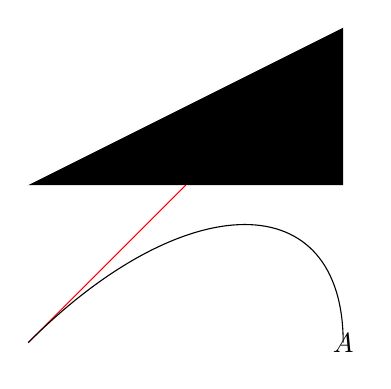
\begin{tikzpicture}[scale=2]
    \draw[red] (0,0) -- +(1,1);
    \path[fill] (2,1) -- (2,2) -- (0,1) -- cycle;
    \draw (0,0) .. controls (1,1) and (2,1) .. (2,0) node {$A$};
  \end{tikzpicture}
\end{texhigh}
\end{examcode}

我们可以自定义注释的显示方式,就是使用 \verb|^^J| 参数:
\begin{examcode}{}
\THSetRange{comment-1}
  [start=\I^\%\s, arguments=\THmN{0}, insert-ending]
  {\THcolor[gray]{0.5}\THSetPlainStyle{cs,color}}%
  [{\color{yellow!70!green}\rmfamily\bfseries \dotfill SC.}]
\THSetRange{comment-2}
  [start=\I^\%e\ , escape, arguments=\THmN{1}, remove-start, use-argument, insert-ending]
  {\THcolor{red}\normalfont \textbf{SP: }}
\THSetRange{comment-3}
  [start=\I^\%a, escape, arguments=m \THmN{1}, remove-start, insert-ending]
  {\def\grab#1{{\rmfamily\bfseries #1:\ }\ignorespaces}%
    \THcolor{purple}\sffamily \grab}
\THSetRange{comment-4}
  [start={\L//\THmS}, arguments=\THmN{0}, insert-ending]
  {\THcolor{green!40!black}\textrm{C style comment: }}

\begin{texhigh}[gobble=auto]
  This is normal % comment(1).
  This is %e Some comment 2.
  %a{comment 3} is the line.
  // This is comment 4.
\end{texhigh}
\end{examcode}

由于 range 在捕获时不能嵌套捕获,使用自定义的注释会导致它内部无法捕获其它 range 了。
一个解决办法是将此 range 设置为 \texttt{escape},然后内部再使用 \cs{texhighverb}。
\begin{examcode}{}
\THSetRange{mycomment}
  % \THmS 表示空格
  [start={\L//\THmS}, escape, arguments=\THmN{1}, remove-start, insert-brace, insert-ending]
  {% \appendpercent “参数处理器”把 \THmP(即“%”)放到参数的前面
    \def\appendpercent#1{\edef\ProcessedArgument{\THmP\unexpanded{#1}}}%
    \DeclareDocumentCommand{\mycommentverb}{>{\appendpercent} v}
      {\texhightext[remove-enabled-ranges={mycomment}]{#1}}%
    % 如果是类别码为 14 且为是第一个“%”就换回 “//\THmS”
    \def\firstComment#1{\if#1\THmP\relax //\THmS \def\firstComment{}\else #1\fi}%
    \THSetClassCH[]{catcode.14}{\firstComment{#1}}%
    \normalfont \mycommentverb}
\begin{texhigh}[gobble=auto, escape-inside=||]
  The |\LaTeX| % comment can be |\emph{highlighted}|.
  // also can be |\emph{highlighted}|, but isn't |\LaTeX|.
\end{texhigh}
\end{examcode}

这个例子展示了如何检测并替换命令中的 \texttt{@@} 符号。
\begin{examcode}[texhigh options={use-ctab=latex3code}]{}
\ExplSyntaxOn
\tl_new:N \l__this_atat_tl
\cs_new:Npn \__this_atat_format:w #1 > 
  {
    \tl_set:Nn \l__this_atat_tl {#1}
    @@ = \l__this_atat_tl
  }
\cs_new:Npn \__this_atat_cs_internal:nn #1#2
  {
    \group_begin:
    \str_set:Nn \l_tmpa_str {#2}
    \tl_replace_once:Nee \l_tmpa_str
      { \tl_to_str:n { _ @@ } } { _ _ \l__this_atat_tl }
    \THcolor { purple } #1 \l_tmpa_str
    \group_end:
  }
\cs_new:Npn \__this_atat_cs_public:nn #1#2
  {
    \group_begin:
    \str_set:Nn \l_tmpa_str {#2}
    \tl_replace_once:Nee \l_tmpa_str
      { \tl_to_str:n { @@ } } { \l__this_atat_tl }
    \THcolor { red } \bfseries #1 \l_tmpa_str
    \group_end:
  }
\THSetRange * {change-at} % 带 * 的不会自动加上 \begingroup \endgroup
  [start={\I^<@@=}, escape, arguments=u{>}, remove-start]
  { \ensuremath{\langle} \__this_atat_format:w }
  [ \ensuremath{\rangle} ]
\THSetClassCS[]{atat-i}{ \__this_atat_cs_internal:nn {#1} {#2} }
\THSetClassCS[]{atat-p}{ \__this_atat_cs_public:nn {#1} {#2} }
\ExplSyntaxOff

\begin{texhigh}[gobble=auto, use-ctab=latex3code,
  cs-category*={atat-i}{_@@}{\THPASS}, % 注意要先匹配 _@@
  cs-category*={atat-p}{@@}{\THPASS},  % 否则只会匹配到 @@
]
  <@@=mycs>
  \tl_new:N \l_@@_code_tl
  \cs_set:Npn \@@_code: { \scan_stop: \l_@@_code_tl }
  <@@=yourcs>
  \tl_new:N \l_@@_code_tl
  \cs_set:Npn \@@_code: { \scan_stop: \l_@@_code_tl }
\end{texhigh}
\end{examcode}

\textsf{texhigh} 默认的定义以及部分命令的用法可参考 \texttt{texhigh.prelude.ths} 文件。

\small

% \bigskip
% \noindent\texhighverb|%%% 以下输出本文源码 %%%|
% \texhighfile[style=tikz.gradient, use-ctab=cjkl3]{\jobname.tex}
% \noindent\texhighverb|%%% 以上是本文源码 %%%|

% \vspace{1cm}
% \noindent\texhighverb|%%%---- File: texhigh.sty ----%%%|
% \texhighfile[use-ctab=latex3code, config-file=config.cfg]{texhigh.sty}

\vspace{1cm}
\noindent\texhighverb|%%%---- File: texhigh.prelude.ths ----%%%|
\IfFileExists{texhigh.prelude.ths.tex}
  {\texhighfile[use-ctab=latexcode]{texhigh.prelude.ths.tex}}
  {\texhighfile[use-ctab=latexcode]{texhigh.prelude.ths}}

% \newpage
% \newgeometry{hmargin=1cm, top=1.5cm, bottom=1.2cm}
% \texhighfile[use-ctab=latex3code,enhanced,font+=\small]{expl3-code.tex}

\end{document}